% Provenance (never printed): cycle 3 "La planete Terre. Les etres vivants
% dans leur environnement" (natural phenomena: volcanoes and earthquakes,
% natural hazards and the behaviour to adopt); see sources/book1/PROVENANCE.md.
% Book 1, grade 4, chapter 2.
\chapter{Gunung Api dan Gempa Bumi: Pengenalan Pertama}\label{ch:g4:volcanoes-earthquakes-first-look}

Pada Senin malam, berita di televisi menayangkan sebuah \omterm{def:g4:volcanoes-earthquakes-first-look:volcano}{gunung api} di
pulau yang jauh. Dalam gelap, air mancur \omterm{def:g3:stones-pebbles-sand:rock}{batuan} jingga yang berpijar
menyembur dari retakan di tanah, dan \omterm{def:g1:landscapes-around-us:water}{sungai-sungai} api mengalir perlahan
menuruni lereng ke \omterm{def:g2:water-on-earth:ocean}{laut}, mendesis dan mengepulkan uap. Pada hari Kamis,
berita menayangkan tempat lain: sebuah kota kecil tempat tanah bergetar
selama setengah menit pada waktu subuh. Cerobong-cerobong asap jatuh ke
jalan, dan sebuah rumah tua tergeser dari fondasinya.

Dua peristiwa yang sangat berbeda. Namun keduanya berasal dari bagian dalam
Bumi yang sangat dalam, dan, seperti yang akan kita lihat, keduanya jauh
lebih sering terjadi di beberapa bagian dunia daripada di bagian lain.

\begin{recall}
\omterm{def:g1:landscapes-around-us:landform}{Gunung}, \omterm{def:g1:landscapes-around-us:landform}{bukit}, \omterm{def:g1:landscapes-around-us:landform}{lembah}, dan \omterm{def:g1:landscapes-around-us:landform}{dataran} adalah bentuk-bentuk permukaan tanah
(\cref{ch:g1:landscapes-around-us}). Daratan Bumi berkumpul dalam tujuh
\omterm{def:g3:continents-and-oceans:continent}{benua}, di antara lima \omterm{def:g2:water-on-earth:ocean}{samudra}; \omterm{def:g2:water-on-earth:ocean}{Samudra} Pasifik adalah \omterm{def:g2:water-on-earth:ocean}{samudra} terbesar
(\cref{ch:g3:continents-and-oceans}).
\end{recall}

\section{Gunung api meletus}

Jauh di bawah kaki kita, Bumi sangat panas. Di beberapa tempat, \omterm{def:g3:stones-pebbles-sand:rock}{batuan} di
bawah sana begitu panas sehingga meleleh. \omterm{def:g3:stones-pebbles-sand:rock}{Batuan} cair ini lebih ringan
daripada \omterm{def:g3:stones-pebbles-sand:rock}{batuan} padat di sekitarnya, sehingga perlahan-lahan naik, seperti
gabus di dalam air. Di tempat \omterm{def:g3:stones-pebbles-sand:rock}{batuan} cair itu menemukan jalan keluar ke
permukaan, lahirlah sebuah \omterm{def:g4:volcanoes-earthquakes-first-look:volcano}{gunung api}.

\begin{definition}[Gunung api]\label{def:g4:volcanoes-earthquakes-first-look:volcano}
Yang disebut \emph{gunung api}\index{gunung api} adalah tempat \omterm{def:g3:stones-pebbles-sand:rock}{batuan} cair
dari bagian dalam Bumi keluar di permukaan, serta \omterm{def:g1:landscapes-around-us:landform}{bukit} atau \omterm{def:g1:landscapes-around-us:landform}{gunung} yang
dibangun di sana oleh \omterm{def:g3:stones-pebbles-sand:rock}{batuan} cair itu, lapis demi lapis.
\end{definition}

\begin{definition}[Letusan, lava, dan abu vulkanik]\label{def:g4:volcanoes-earthquakes-first-look:eruption}
Yang disebut \emph{letusan}\index{letusan} adalah saat sebuah \omterm{def:g4:volcanoes-earthquakes-first-look:volcano}{gunung api}
menyemburkan \omterm{def:g3:stones-pebbles-sand:rock}{batuan} cair, abu, dan gas. Yang disebut \emph{lava}\index{lava}
adalah \omterm{def:g3:stones-pebbles-sand:rock}{batuan} cair yang tercurah ke permukaan; lava mengalir, lalu
mendingin dan mengeras menjadi \omterm{def:g3:stones-pebbles-sand:rock}{batuan} baru. Yang disebut
\emph{abu vulkanik}\index{abu vulkanik} adalah kepingan-kepingan kecil
\omterm{def:g3:stones-pebbles-sand:rock}{batuan} dan kaca yang diembuskan ke udara oleh letusan; abu itu jatuh
kembali seperti \omterm{def:g4:clouds-rain-snow:precipitation}{salju} kelabu.
\end{definition}

\begin{omfigure}
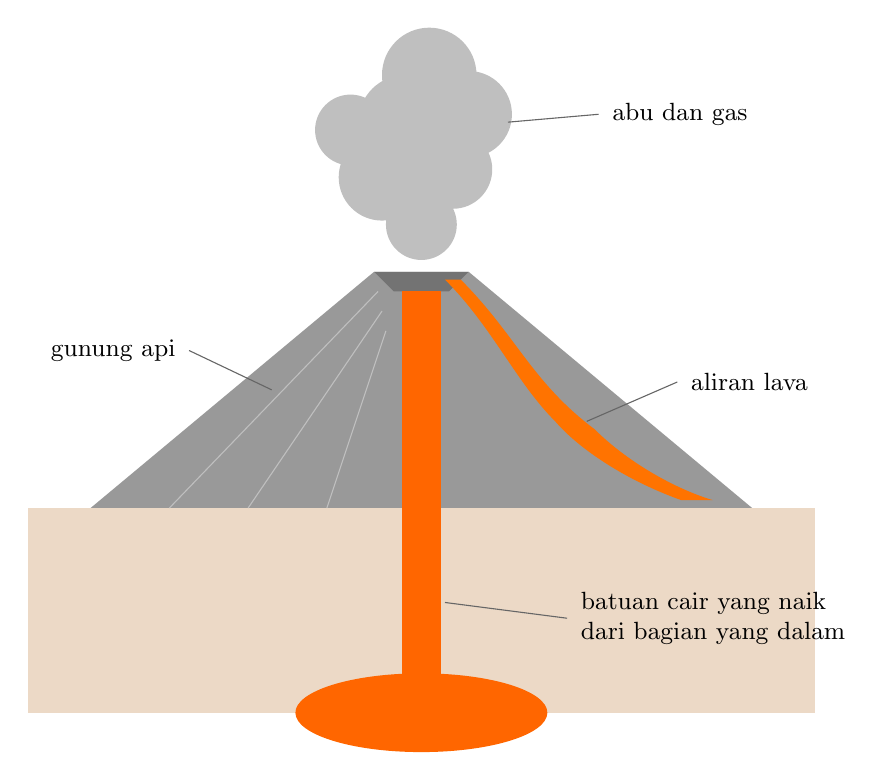
\begin{tikzpicture}[font=\small]
  % ground and deep rock
  \fill[brown!30] (-5,-2.6) rectangle (5,0);
  % the volcano
  \fill[black!40] (-4.2,0) -- (-0.6,3.0) -- (0.6,3.0) -- (4.2,0) -- cycle;
  \fill[black!55] (-0.6,3.0) -- (-0.35,2.75) -- (0.35,2.75) -- (0.6,3.0) -- cycle;
  % layers inside the cone
  \foreach \k in {1,2,3}
    \draw[black!25] (-4.2+1.0*\k,0) -- (-0.6+0.05*\k,3.0-0.25*\k);
  % molten rock rising from deep below
  \fill[orange!80!red] (-0.25,-2.6) -- (-0.25,2.75) -- (0.25,2.75) -- (0.25,-2.6) -- cycle;
  \fill[orange!80!red] (0,-2.6) ellipse (1.6 and 0.5);
  % lava flow on the right flank
  \fill[orange!90!red] (0.5,2.9) .. controls (1.2,2.2) and (1.4,1.6) .. (2.2,1.0)
    .. controls (2.6,0.6) and (3.2,0.25) .. (3.7,0.1) -- (3.3,0.1)
    .. controls (2.6,0.35) and (2.0,0.75) .. (1.7,1.1)
    .. controls (1.2,1.6) and (0.9,2.3) .. (0.3,2.9) -- cycle;
  % ash and gas cloud
  \foreach \x/\y/\r in {0/3.6/0.45, -0.5/4.2/0.55, 0.4/4.3/0.5, -0.2/4.9/0.6, 0.6/5.0/0.55, -0.9/4.8/0.45, 0.1/5.5/0.6}
    \fill[black!25] (\x,\y) circle (\r);
  % labels
  \node[anchor=west] at (2.3,5.0) {abu dan gas};
  \draw[black!60] (2.25,5.0) -- (1.1,4.9);
  \node[anchor=west] at (3.3,1.6) {aliran lava};
  \draw[black!60] (3.25,1.6) -- (2.1,1.1);
  \node[anchor=east] at (-3.0,2.0) {gunung api};
  \draw[black!60] (-2.95,2.0) -- (-1.9,1.5);
  \node[anchor=west, align=left] at (1.9,-1.4) {batuan cair yang naik\\dari bagian yang dalam};
  \draw[black!60] (1.85,-1.4) -- (0.3,-1.2);
\end{tikzpicture}

{\small \omterm{def:g4:volcanoes-earthquakes-first-look:volcano}{Gunung api} yang sedang meletus (digambar, tidak berskala). \omterm{def:g3:stones-pebbles-sand:rock}{Batuan}
cair naik dari bagian yang dalam dan keluar di puncak: \omterm{def:g3:stones-pebbles-sand:rock}{batuan} itu mengalir
turun sebagai \omterm{def:g4:volcanoes-earthquakes-first-look:eruption}{lava}, sementara abu dan gas diembuskan ke langit. Setiap
\omterm{def:g4:volcanoes-earthquakes-first-look:eruption}{letusan} menambahkan lapisan baru pada \omterm{def:g1:landscapes-around-us:landform}{gunung} itu.}
\label{fig:g4:volcanoes-earthquakes-first-look:volcano}
\end{omfigure}

Tidak semua \omterm{def:g4:volcanoes-earthquakes-first-look:eruption}{letusan} tampak sama. Pada sebagian \omterm{def:g4:volcanoes-earthquakes-first-look:eruption}{letusan}, \omterm{def:g4:volcanoes-earthquakes-first-look:eruption}{lavanya} encer: \omterm{def:g4:volcanoes-earthquakes-first-look:eruption}{lava}
itu tercurah dengan tenang dalam \omterm{def:g1:landscapes-around-us:water}{sungai-sungai} yang berpijar yang bisa
mengalir berkilo-kilometer, kadang-kadang sampai ke \omterm{def:g2:water-on-earth:ocean}{laut}. Pada \omterm{def:g4:volcanoes-earthquakes-first-look:eruption}{letusan}
yang lain, \omterm{def:g3:stones-pebbles-sand:rock}{batuan} cairnya kental dan penuh gas, seperti sebotol minuman
bersoda yang dikocok: ketika menyembur keluar, \omterm{def:g3:stones-pebbles-sand:rock}{batuan} itu meledak menjadi
tiang abu raksasa yang naik tinggi ke langit.

\begin{omfigure}
\begin{minipage}[b]{0.56\linewidth}\centering
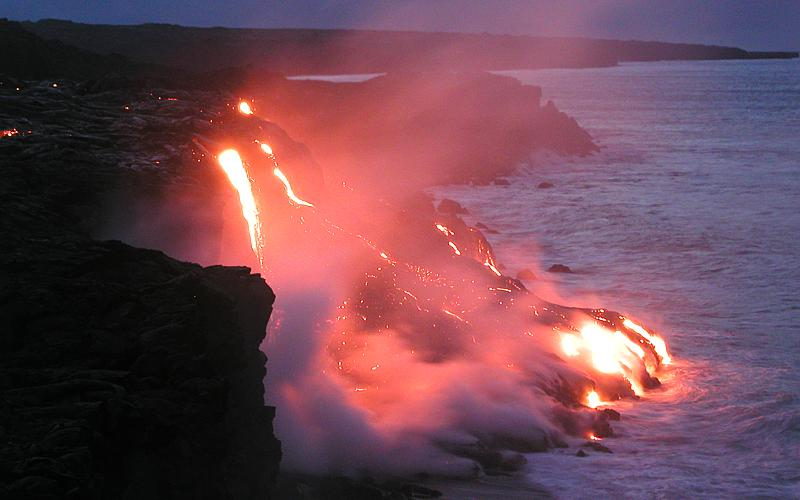
\includegraphics[width=\linewidth]{images/book1/g4-lava-ocean.jpg}

{\small \omterm{def:g4:volcanoes-earthquakes-first-look:eruption}{Letusan} yang encer: \omterm{def:g4:volcanoes-earthquakes-first-look:eruption}{lava} mengalir menuruni tebing \omterm{def:g2:water-on-earth:ocean}{laut} ke \omterm{def:g2:water-on-earth:ocean}{samudra},
di Hawaii. Foto: USGS Hawaiian Volcano Observatory (domain publik).}
\end{minipage}\hfill
\begin{minipage}[b]{0.4\linewidth}\centering
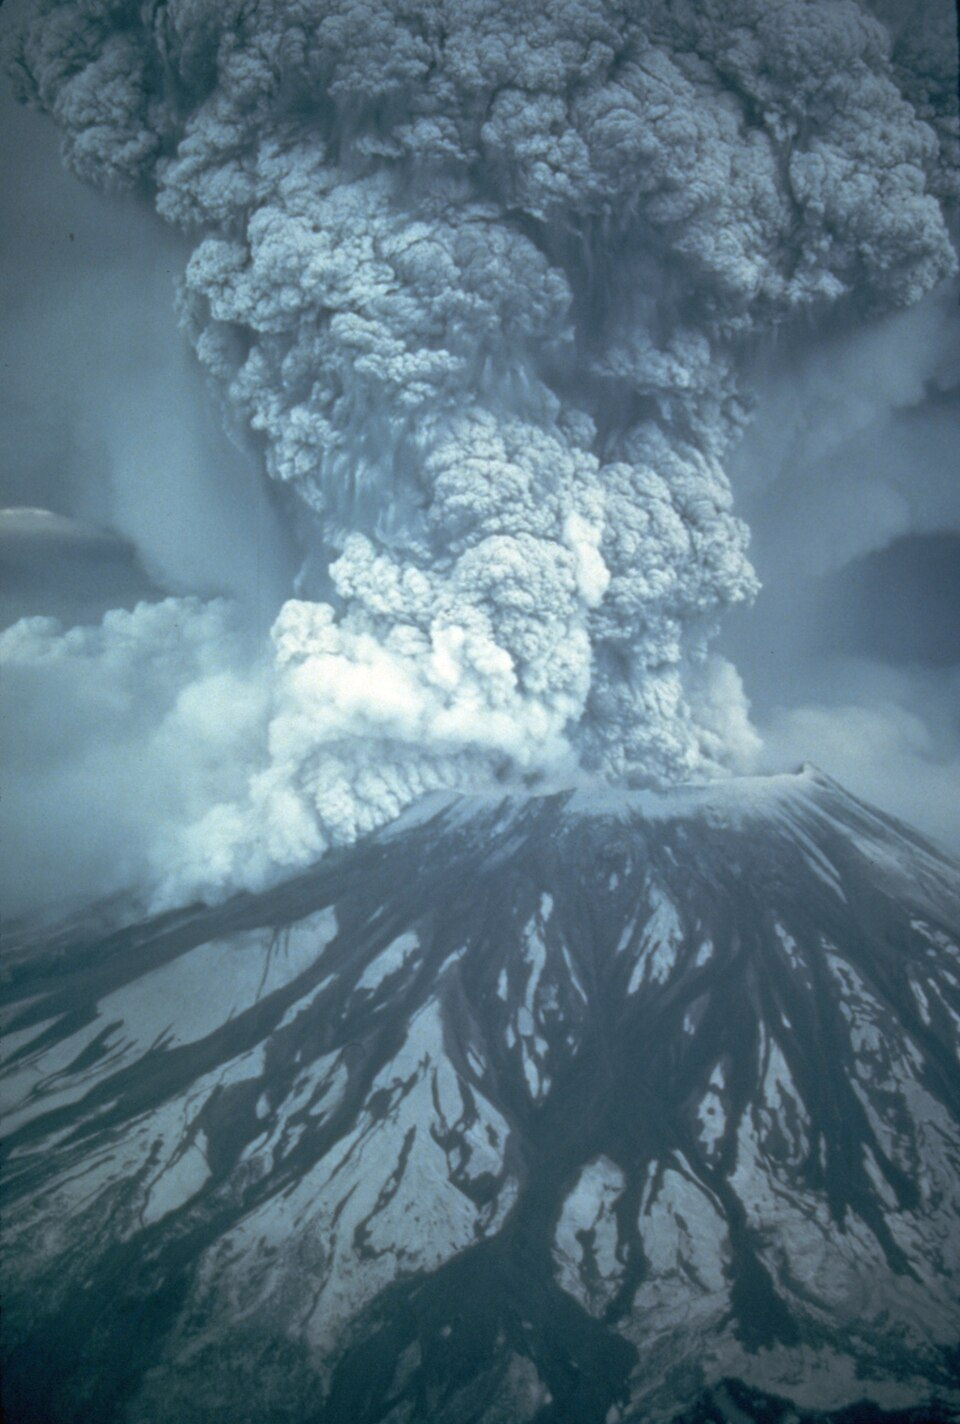
\includegraphics[width=0.78\linewidth]{images/book1/g4-st-helens.jpg}

{\small \omterm{def:g4:volcanoes-earthquakes-first-look:eruption}{Letusan} yang eksplosif: Gunung St.~Helens, Amerika Serikat, 18~Mei
1980. Foto: Austin Post, USGS (domain publik).}
\end{minipage}
% ledger: usgs:pu-oo-ocean, usgs:msh-1980
\label{fig:g4:volcanoes-earthquakes-first-look:two-eruptions}
\end{omfigure}

\begin{example}[Gunung St.~Helens, 1980]\label{ex:g4:volcanoes-earthquakes-first-look:st-helens}
Pada musim semi tahun 1980, sebuah tonjolan tumbuh di sisi Gunung
St.~Helens, karena \omterm{def:g3:stones-pebbles-sand:rock}{batuan} cair mendesak naik di dalam \omterm{def:g1:landscapes-around-us:landform}{gunung} itu. Pada
pagi hari tanggal 18~Mei, gempa kecil mengguncang \omterm{def:g1:landscapes-around-us:landform}{gunung} itu, tonjolan itu
meluncur dalam tanah longsor raksasa, dan \omterm{def:g4:volcanoes-earthquakes-first-look:volcano}{gunung api} itu meledak ke samping
dan ke atas. Bagian puncak \omterm{def:g1:landscapes-around-us:landform}{gunung} setinggi 400~meter lenyap: puncaknya
berubah menjadi kawah yang sangat besar.
% ledger: usgs:msh-1980
\end{example}

\section{Tanah berguncang}

\omterm{def:g3:stones-pebbles-sand:rock}{Batuan} jauh di bawah kaki kita tidak benar-benar diam. Sangat perlahan,
\omterm{def:g3:stones-pebbles-sand:rock}{batuan} itu didorong dan ditarik. \omterm{def:g3:stones-pebbles-sand:rock}{Batuan} itu sedikit melengkung, seperti
penggaris yang kamu tekan dari kedua ujungnya --- sampai, tiba-tiba,
\omterm{def:g3:stones-pebbles-sand:rock}{batuan} itu patah dan bergeser. Sentakannya membuat tanah berguncang sampai
berkilo-kilometer di sekelilingnya.

\begin{definition}[Gempa bumi]\label{def:g4:volcanoes-earthquakes-first-look:earthquake}
Yang disebut \emph{gempa bumi}\index{gempa bumi} adalah guncangan tanah yang
tiba-tiba, yang disebabkan oleh \omterm{def:g3:stones-pebbles-sand:rock}{batuan} yang patah dan bergeser, jauh di
bawah tanah.
\end{definition}

\omterm{def:g4:volcanoes-earthquakes-first-look:earthquake}{Gempa bumi} biasanya hanya berlangsung beberapa detik, kadang-kadang satu
atau dua menit untuk yang terbesar. Kebanyakan \omterm{def:g4:volcanoes-earthquakes-first-look:earthquake}{gempa bumi} begitu kecil
sehingga tidak ada yang merasakannya: hanya alat ukur yang mencatatnya.
Gempa yang kuat bisa membuat tanah bergelombang seperti geladak kapal,
meretakkan jalan, dan merobohkan dinding dan rumah.

\begin{omfigure}
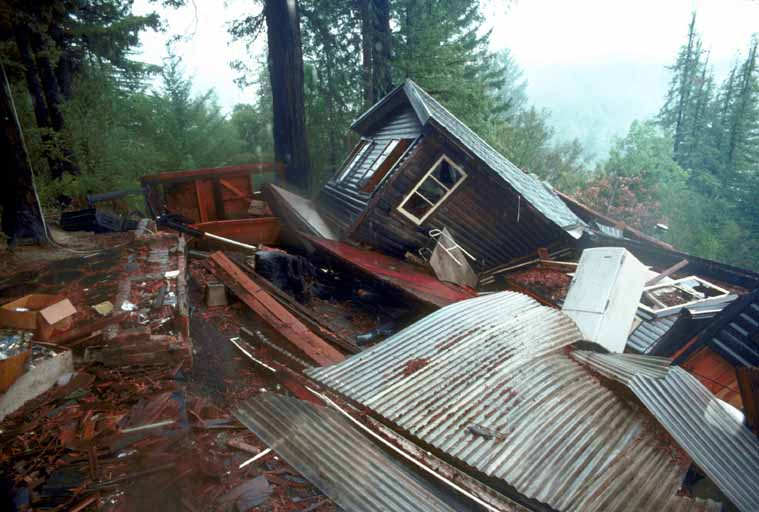
\includegraphics[width=0.55\linewidth]{images/book1/g4-loma-prieta-house.jpg}

{\small Setelah \omterm{def:g4:volcanoes-earthquakes-first-look:earthquake}{gempa bumi} yang kuat di California pada tahun 1989: rumah
kayu ini terlempar ke samping dari alas betonnya. Foto: J.~K.~Nakata, USGS
(domain publik).}
% ledger: usgs:loma-prieta-house
\end{omfigure}

\begin{remark}[Seberapa sering?]\label{rem:g4:volcanoes-earthquakes-first-look:how-often}
Para ahli geologi menyimpan daftar semua \omterm{def:g4:volcanoes-earthquakes-first-look:earthquake}{gempa bumi} besar di Bumi. Selama
50 tahun dari 1976 sampai 2025, daftar itu mencatat 7\,031 gempa besar
(cukup kuat untuk merusak bangunan di dekatnya): sekitar 141 dalam
setahun, atau hampir 3 setiap minggu. Yang paling besar, yang bisa
menghancurkan seluruh kota, sekitar 14 dalam setahun. Di seluruh Bumi yang
sama, sekitar 1\,200 \omterm{def:g4:volcanoes-earthquakes-first-look:volcano}{gunung api} sudah meletus dalam kira-kira dua belas
ribu tahun terakhir.
% ledger: data:usgs-comcat, data:gvp
\end{remark}

\section{Di mana gunung api dan gempa bumi terjadi}

Jika \omterm{def:g4:volcanoes-earthquakes-first-look:volcano}{gunung api} dan \omterm{def:g4:volcanoes-earthquakes-first-look:earthquake}{gempa bumi} terjadi di sembarang tempat secara acak,
titik-titik pada \omterm{def:g3:continents-and-oceans:world-map}{peta dunia} akan tersebar merata di atasnya. Ternyata
tidak.

\omterm{def:g2:drawing-to-map:map}{Peta} di bawah ini menunjukkan pola yang mencolok. Kebanyakan \omterm{def:g4:volcanoes-earthquakes-first-look:volcano}{gunung api} dan
kebanyakan \omterm{def:g4:volcanoes-earthquakes-first-look:earthquake}{gempa bumi} besar terletak di sabuk-sabuk yang panjang dan
sempit. Sabuk yang paling panjang melingkari \omterm{def:g2:water-on-earth:ocean}{Samudra} Pasifik: dari Selandia
Baru naik melalui Indonesia, Filipina, dan Jepang, menyeberang ke Alaska,
lalu terus turun di sepanjang pantai barat benua Amerika sampai ke ujung
Chili. Karena \omterm{def:g4:volcanoes-earthquakes-first-look:volcano}{gunung apinya} yang banyak, sabuk ini sering disebut
``Cincin Api''.

\begin{example}[Menghitung pada peta]\label{ex:g4:volcanoes-earthquakes-first-look:shares}
Kita menghitung titik-titik yang terletak di dalam cincin yang diarsir
(dalam jarak 500~kilometer dari garis tengahnya). Dari 1\,214 \omterm{def:g4:volcanoes-earthquakes-first-look:volcano}{gunung api},
837 berada di dalam cincin: sekitar 2 dari setiap 3. Dari 696 \omterm{def:g4:volcanoes-earthquakes-first-look:earthquake}{gempa bumi}
yang sangat besar, 532 berada di dalam cincin: sekitar 3 dari setiap 4.
Cincin itu hanya mencakup sebagian kecil Bumi, tetapi menampung sebagian
besar \omterm{def:g4:volcanoes-earthquakes-first-look:volcano}{gunung api} dan \omterm{def:g4:volcanoes-earthquakes-first-look:earthquake}{gempa buminya}.
% ledger: data:gvp, data:usgs-comcat
\end{example}

\begin{omfigure}
\begin{tikzpicture}
\begin{axis}[ommap, width=\linewidth, xtick=\empty, ytick=\empty, grid=none,
    legend style={font=\scriptsize, at={(0.5,-0.02)}, anchor=north,
      draw=none, legend columns=3, /tikz/every even column/.append style={column sep=6pt}},
    legend cell align=left]
  \addplot[fill=omHypsLandA!85!black, draw=black!45, line width=0.2pt, forget plot]
    table {figdata/out/shared-geo-land.dat};
  \addplot[orange!80!black, opacity=0.35, line width=9pt, line cap=round, line join=round]
    table {figdata/out/grade-4-ring_of_fire-ring.dat};
  \addlegendentry{cincin Samudra Pasifik}
  \addplot[only marks, mark=triangle*, mark size=1.3pt, red!75!black]
    table[x=lon, y=lat] {figdata/out/grade-4-ring_of_fire-volcanoes.dat};
  \addlegendentry{gunung api (12\,000 tahun terakhir)}
  \addplot[only marks, mark=*, mark size=1.0pt, black, fill opacity=0.6]
    table[x=lon, y=lat] {figdata/out/grade-4-ring_of_fire-quakes7.dat};
  \addlegendentry{gempa sangat besar (1976--2025)}
\end{axis}
\end{tikzpicture}

{\small \omterm{def:g4:volcanoes-earthquakes-first-look:volcano}{Gunung api} yang sudah meletus dalam kira-kira dua belas ribu tahun
terakhir, dan gempa-gempa bumi yang paling besar pada 1976--2025.
Kebanyakan terletak di sepanjang cincin rangkaian pulau dan pegunungan di
sekeliling \omterm{def:g2:water-on-earth:ocean}{Samudra} Pasifik (diarsir). Data: Smithsonian Global Volcanism
Program; katalog \omterm{def:g4:volcanoes-earthquakes-first-look:earthquake}{gempa bumi} U.S. Geological Survey; garis pantai Natural
Earth.}
\label{fig:g4:volcanoes-earthquakes-first-look:map}
% ledger: data:gvp, data:usgs-comcat, data:ne-land
\end{omfigure}

Sabuk-sabuk lain lebih kecil: satu melintasi Eropa selatan dan Asia, dari
\omterm{def:g2:water-on-earth:ocean}{Laut} Tengah sampai ke Himalaya; sabuk-sabuk lainnya membentang di tengah
\omterm{def:g2:water-on-earth:ocean}{samudra}, tempat \omterm{def:g4:volcanoes-earthquakes-first-look:volcano}{gunung-gunung api} tersembunyi di bawah air. Beberapa
tempat, seperti Hawaii, mempunyai \omterm{def:g4:volcanoes-earthquakes-first-look:volcano}{gunung api} yang jauh dari sabuk mana pun.
Mengapa sabuk-sabuk itu berada di tempatnya adalah pertanyaan untuk
\cref{ch:g7:plate-tectonics}: jawabannya menjelaskan bentuk seluruh \omterm{def:g2:drawing-to-map:map}{peta}.

\section{Tetap selamat}

Tidak seorang pun bisa menghentikan \omterm{def:g4:volcanoes-earthquakes-first-look:eruption}{letusan} atau \omterm{def:g4:volcanoes-earthquakes-first-look:earthquake}{gempa bumi}. Tetapi
mengetahui apa yang harus dilakukan menyelamatkan nyawa.

\begin{omfigure}
\begin{tikzpicture}[font=\small, line cap=round, line join=round]
  % --- panel 1: DROP onto hands and knees
  \begin{scope}
    \draw[black!30] (-0.2,0) -- (2.8,0);
    \fill[omDef] (0.62,0.98) circle (0.21);
    \draw[omDef, line width=2.2pt] (0.88,0.98) -- (2.0,0.95);
    \draw[omDef, line width=2pt] (0.95,0.96) -- (0.95,0.05);
    \draw[omDef, line width=2pt] (2.0,0.95) -- (1.98,0.08) -- (2.65,0.08);
    \node[font=\bfseries] at (1.3,-0.45) {MERUNDUK};
    \node[font=\scriptsize, align=center] at (1.3,-0.95) {bertumpu pada\\tangan dan lutut};
  \end{scope}
  % --- panel 2: COVER under a table
  \begin{scope}[xshift=4cm]
    \draw[black!30] (-0.2,0) -- (2.8,0);
    \fill[brown!60!black] (-0.1,1.45) rectangle (2.7,1.6);
    \draw[brown!60!black, line width=2pt] (0.1,1.45) -- (0.1,0) (2.5,1.45) -- (2.5,0);
    \fill[omDef] (0.75,0.95) circle (0.2);
    \draw[omDef, line width=2.2pt] (0.95,0.85) -- (1.95,0.8);
    \draw[omDef, line width=2pt] (1.9,0.8) -- (1.65,0.05) -- (2.25,0.05);
    \draw[omDef, line width=2pt] (1.0,0.85) -- (0.7,1.2) -- (0.5,0.95);
    \node[font=\bfseries] at (1.3,-0.45) {BERLINDUNG};
    \node[font=\scriptsize, align=center] at (1.3,-0.95) {lindungi kepala dan leher,\\di bawah meja yang kokoh};
  \end{scope}
  % --- panel 3: HOLD ON to the table leg
  \begin{scope}[xshift=8cm]
    \draw[black!30] (-0.2,0) -- (2.8,0);
    \fill[brown!60!black] (-0.1,1.45) rectangle (2.7,1.6);
    \draw[brown!60!black, line width=2pt] (0.1,1.45) -- (0.1,0) (2.5,1.45) -- (2.5,0);
    \fill[omDef] (0.75,0.95) circle (0.2);
    \draw[omDef, line width=2.2pt] (0.95,0.85) -- (1.95,0.8);
    \draw[omDef, line width=2pt] (1.9,0.8) -- (1.65,0.05) -- (2.25,0.05);
    \draw[omDef, line width=2pt] (1.0,0.85) -- (0.7,1.2) -- (0.5,0.95);
    \draw[omDef, line width=2pt] (1.0,0.8) -- (0.45,0.6) -- (0.12,0.65);
    \node[font=\bfseries] at (1.3,-0.45) {BERPEGANGAN};
    \node[font=\scriptsize, align=center] at (1.3,-0.95) {pada meja sampai\\guncangan berhenti};
  \end{scope}
\end{tikzpicture}

{\small Apa yang harus dilakukan segera setelah tanah mulai berguncang:
merunduk, berlindung, dan berpegangan.}
\label{fig:g4:volcanoes-earthquakes-first-look:drop-cover}
% ledger: shakeout:dch
\end{omfigure}

\begin{safety}
\textbf{Saat \omterm{def:g4:volcanoes-earthquakes-first-look:earthquake}{gempa bumi}.} Segera setelah kamu merasakan tanah berguncang:
\textbf{merunduklah} dengan bertumpu pada tangan dan lutut;
\textbf{lindungilah} kepala dan lehermu dengan lengan, dan merangkaklah ke
bawah meja yang kokoh jika ada di dekatmu; \textbf{berpeganganlah} pada
meja itu sampai guncangan berhenti. Jangan berlari ke luar selagi tanah
berguncang, dan jangan berdiri di ambang pintu: pecahan kaca dan
benda-benda yang jatuh adalah bahaya yang utama. Ketika guncangan
berhenti, tinggalkan gedung dengan tenang, seperti yang kamu latih dalam
latihan di sekolah.

\textbf{Di dekat \omterm{def:g4:volcanoes-earthquakes-first-look:volcano}{gunung api}.} Para ilmuwan mengawasi \omterm{def:g4:volcanoes-earthquakes-first-look:volcano}{gunung-gunung api} yang
mungkin bangun. Jika mereka memperingatkan bahwa \omterm{def:g4:volcanoes-earthquakes-first-look:eruption}{letusan} akan terjadi,
pihak berwenang meminta penduduk meninggalkan daerah itu. Ikutilah
petunjuk mereka segera, dan jangan pernah mendekat untuk menonton.
\end{safety}
% ledger: shakeout:dch

\begin{omfigure}
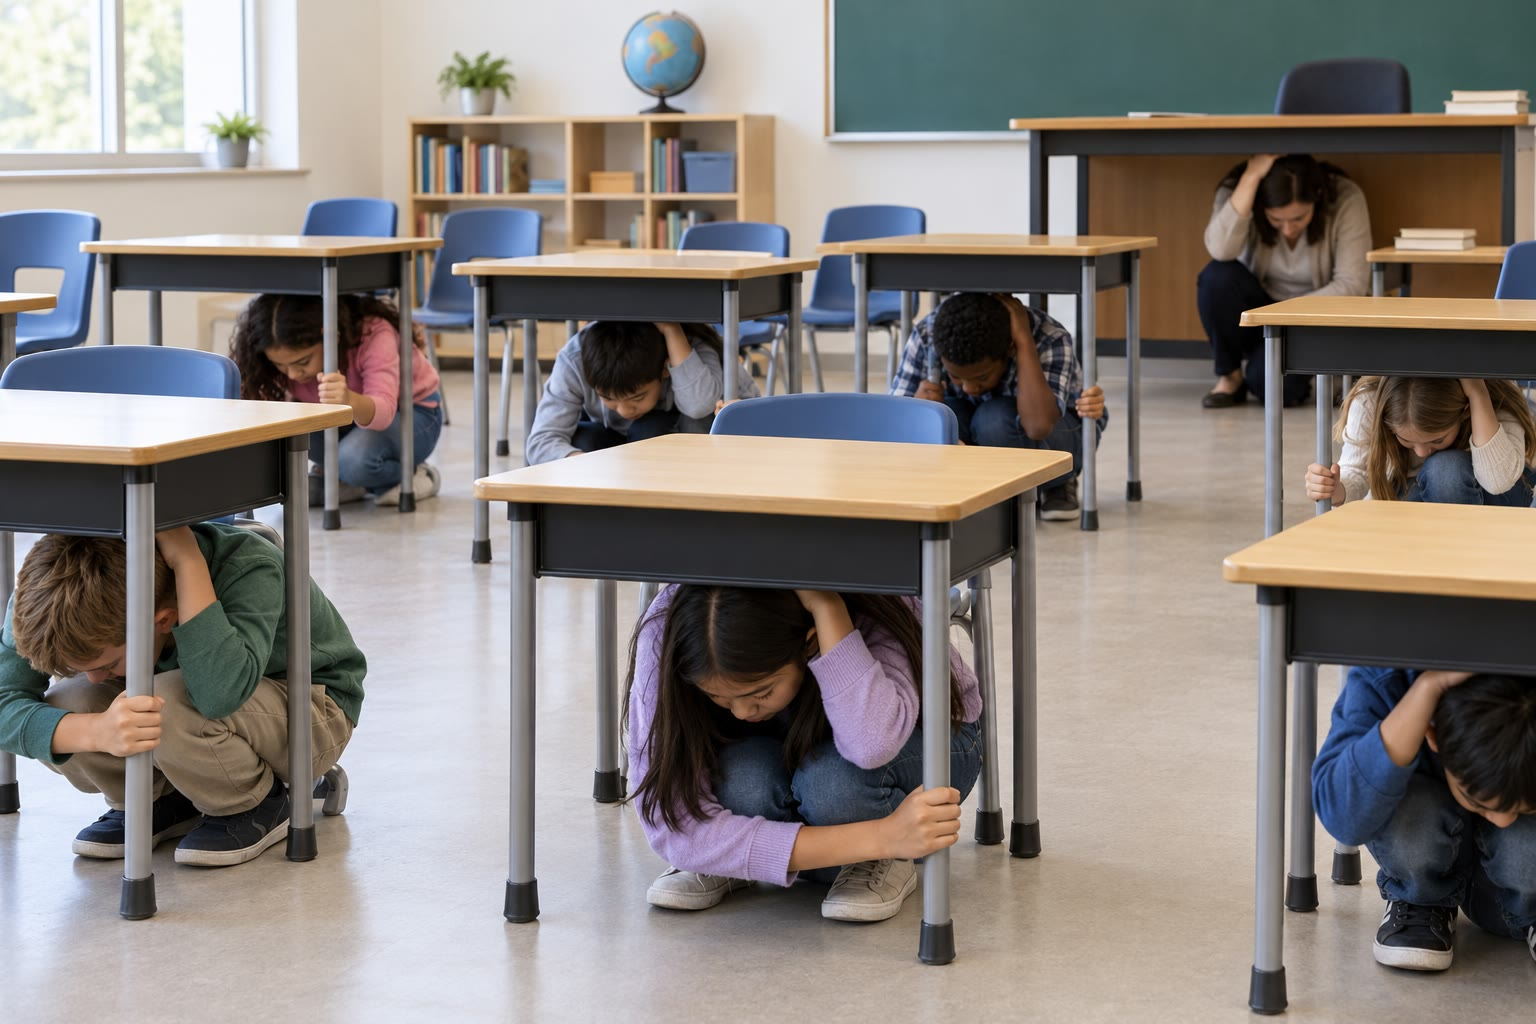
\includegraphics[width=0.55\linewidth]{images/book1/ai/g4-earthquake-drill.jpg}

{\small Latihan \omterm{def:g4:volcanoes-earthquakes-first-look:earthquake}{gempa bumi}: para murid berlatih ``merunduk, berlindung, dan
berpegangan'' di bawah meja mereka.}
\end{omfigure}

\section{Latihan}

\begin{exercise}[$\star$]\label{exo:g4:volcanoes-earthquakes-first-look:1}
\omterm{def:g4:volcanoes-earthquakes-first-look:eruption}{Lava}, abu, atau gas? (a) \omterm{def:g1:landscapes-around-us:water}{sungai} \omterm{def:g3:stones-pebbles-sand:rock}{batuan} cair yang berpijar yang mengalir
menuruni lereng; (b) kepingan-kepingan kecil \omterm{def:g3:stones-pebbles-sand:rock}{batuan} yang diembuskan ke
langit, yang jatuh kembali seperti \omterm{def:g4:clouds-rain-snow:precipitation}{salju} kelabu; (c) sesuatu yang tidak
terlihat yang keluar dari \omterm{def:g4:volcanoes-earthquakes-first-look:volcano}{gunung api} bersama abu.
\end{exercise}

\begin{exercise}[$\star$]\label{exo:g4:volcanoes-earthquakes-first-look:2}
Apa itu \omterm{def:g4:volcanoes-earthquakes-first-look:earthquake}{gempa bumi}? Apakah \omterm{def:g4:volcanoes-earthquakes-first-look:earthquake}{gempa bumi} berlangsung berjam-jam, atau beberapa detik?
\end{exercise}

\begin{exercise}[$\star$]\label{exo:g4:volcanoes-earthquakes-first-look:3}
Urutkan ketiga langkah ini: berpegangan; merunduk; berlindung.
\end{exercise}

\begin{exercise}[$\star$]\label{exo:g4:volcanoes-earthquakes-first-look:4}
Pada \omterm{def:g2:drawing-to-map:map}{peta} di halaman~\pageref{fig:g4:volcanoes-earthquakes-first-look:map},
di sekeliling \omterm{def:g2:water-on-earth:ocean}{samudra} manakah kebanyakan \omterm{def:g4:volcanoes-earthquakes-first-look:volcano}{gunung api} terletak?
\end{exercise}

\begin{exercise}[$\star$]\label{exo:g4:volcanoes-earthquakes-first-look:5}
Benar atau salah? (a) Kebanyakan \omterm{def:g4:volcanoes-earthquakes-first-look:earthquake}{gempa bumi} terlalu kecil untuk dirasakan.
(b) \omterm{def:g4:volcanoes-earthquakes-first-look:eruption}{Lava} tetap cair selamanya. (c) Ketika tanah berguncang, hal yang paling
aman adalah berlari ke luar.
\end{exercise}

\begin{exercise}[$\star$]\label{exo:g4:volcanoes-earthquakes-first-look:6}
Lihatlah gambar \omterm{def:g4:volcanoes-earthquakes-first-look:volcano}{gunung api} di halaman~\pageref{fig:g4:volcanoes-earthquakes-first-look:volcano}.
Dari mana \omterm{def:g3:stones-pebbles-sand:rock}{batuan} cair itu berasal? Di mana \omterm{def:g3:stones-pebbles-sand:rock}{batuan} itu keluar?
\end{exercise}

\begin{exercise}[$\star\star$]\label{exo:g4:volcanoes-earthquakes-first-look:7}
Pada \omterm{def:g2:drawing-to-map:map}{peta}, carilah: (a) sebuah negara di benua Amerika yang mempunyai
banyak \omterm{def:g4:volcanoes-earthquakes-first-look:volcano}{gunung api} di sepanjang wilayahnya; (b) sekelompok pulau di tengah
\omterm{def:g2:water-on-earth:ocean}{Samudra} Pasifik, dengan \omterm{def:g4:volcanoes-earthquakes-first-look:volcano}{gunung-gunung api}, yang tidak berada di cincin itu.
\end{exercise}

\begin{exercise}[$\star\star$]\label{exo:g4:volcanoes-earthquakes-first-look:8}
Sekitar 141 \omterm{def:g4:volcanoes-earthquakes-first-look:earthquake}{gempa bumi} besar terjadi dalam setahun. Kira-kira berapa
banyaknya dalam sebulan? (Setahun ada 12 bulan; berikan bilangan bulat.)
\end{exercise}

\begin{exercise}[$\star\star$]\label{exo:g4:volcanoes-earthquakes-first-look:9}
Sekitar 3 dari setiap 4 \omterm{def:g4:volcanoes-earthquakes-first-look:earthquake}{gempa bumi} yang sangat besar terjadi di dalam
cincin di sekeliling \omterm{def:g2:water-on-earth:ocean}{Samudra} Pasifik. Dari 20 \omterm{def:g4:volcanoes-earthquakes-first-look:earthquake}{gempa bumi} yang sangat besar,
kira-kira berapa yang kamu perkirakan terjadi di dalam cincin? Dan berapa
di luarnya?
\end{exercise}

\begin{exercise}[$\star\star$]\label{exo:g4:volcanoes-earthquakes-first-look:10}
Selama latihan \omterm{def:g4:volcanoes-earthquakes-first-look:earthquake}{gempa bumi}, Leo berlari dan berdiri di ambang pintu kelas.
Apa yang seharusnya ia lakukan, dan mengapa?
\end{exercise}

\begin{exercise}[$\star\star\star$]\label{exo:g4:volcanoes-earthquakes-first-look:11}
Dari 1\,214 \omterm{def:g4:volcanoes-earthquakes-first-look:volcano}{gunung api} pada \omterm{def:g2:drawing-to-map:map}{peta}, 837 berada di dalam cincin di sekeliling
\omterm{def:g2:water-on-earth:ocean}{Samudra} Pasifik. Berapa yang berada di luarnya? Apakah ``sekitar 2 dari 3''
cara yang baik untuk menggambarkan bagian yang berada di dalam cincin?
(Petunjuk: berapa dua pertiga dari 1\,200?)
\end{exercise}
